% Graphs Appendix (PDF)
% Compile:
%   pdflatex graphs_report.tex
%
% Notes:
% - This document is graphs/tables only (quantitative + qualitative).
% - It reuses the same key numbers as `final_report.tex`.

\documentclass[11pt]{article}

\usepackage[margin=1in]{geometry}
\usepackage{microtype}
\usepackage{amsmath}
\usepackage{amssymb}
\usepackage{booktabs}
\usepackage{graphicx}
\usepackage{siunitx}
\usepackage{xcolor}
\usepackage{hyperref}
\hypersetup{
  colorlinks=true,
  linkcolor=blue!60!black,
  urlcolor=blue!60!black
}
\usepackage{tikz}
\usetikzlibrary{positioning,arrows.meta}
\usepackage{pgfplots}
\usepackage{pgfplotstable}
\usepackage{subcaption}

\pgfplotsset{compat=1.18}
\sisetup{detect-weight=true, detect-family=true}
\setlength{\parindent}{0pt}

% -----------------------------
% Key numbers (copied from final_report.tex)
% -----------------------------
\newcommand{\NTotal}{597{,}928}
\newcommand{\NTrain}{418{,}549}
\newcommand{\NVal}{89{,}689}
\newcommand{\NTest}{89{,}690}

\newcommand{\AnnParams}{629{,}340}
\newcommand{\AnnRandRmseMean}{0.1420}
\newcommand{\AnnRandRmseStd}{0.0036}
\newcommand{\AnnRandAccMean}{92.64}
\newcommand{\AnnRandAccStd}{0.31}
\newcommand{\AnnTimeRmseMean}{0.3146}
\newcommand{\AnnTimeRmseStd}{0.0365}
\newcommand{\AnnTimeAccMean}{82.78}
\newcommand{\AnnTimeAccStd}{2.35}

\newcommand{\HedRandRmseMean}{0.2446}
\newcommand{\HedRandRmseStd}{0.0030}
\newcommand{\HedRandAccMean}{87.76}
\newcommand{\HedRandAccStd}{0.10}
\newcommand{\HedTimeRmseMean}{0.5947}
\newcommand{\HedTimeRmseStd}{0.0162}
\newcommand{\HedTimeAccMean}{69.35}
\newcommand{\HedTimeAccStd}{1.09}

\newcommand{\DeepRandRmseMean}{0.1708}
\newcommand{\DeepRandRmseStd}{0.0085}
\newcommand{\DeepRandAccMean}{91.22}
\newcommand{\DeepRandAccStd}{0.51}
\newcommand{\DeepTimeRmseMean}{0.3533}
\newcommand{\DeepTimeRmseStd}{0.0107}
\newcommand{\DeepTimeAccMean}{75.74}
\newcommand{\DeepTimeAccStd}{1.51}

\newcommand{\NaiveMeanRmse}{0.5618}
\newcommand{\NaiveMeanAcc}{66.10}

\newcommand{\FmParams}{123{,}302}
\newcommand{\FmTestRmse}{0.2169}
\newcommand{\FmTestAcc}{89.34}
\newcommand{\FmTimeTestRmse}{0.5090}
\newcommand{\FmTimeTestAcc}{82.37}

\newcommand{\TabnetParams}{839{,}892}
\newcommand{\TabnetTestRmse}{0.3907}
\newcommand{\TabnetTestAcc}{78.11}
\newcommand{\TabnetTimeTestRmse}{0.4349}
\newcommand{\TabnetTimeTestAcc}{75.08}

\newcommand{\TabtrParams}{681{,}473}
\newcommand{\TabtrTestRmse}{0.1997}
\newcommand{\TabtrTestAcc}{88.97}
\newcommand{\TabtrTimeTestRmse}{0.2730}
\newcommand{\TabtrTimeTestAcc}{79.06}

\newcommand{\FtParams}{617{,}409}
\newcommand{\FtTestRmse}{0.1669}
\newcommand{\FtTestAcc}{91.42}
\newcommand{\FtTimeTestRmse}{0.2604}
\newcommand{\FtTimeTestAcc}{87.71}

\newcommand{\BasicAnnTestRmse}{0.3088}
\newcommand{\BasicAnnTestAcc}{82.54}
\newcommand{\BasicHedTestRmse}{0.4722}
\newcommand{\BasicHedTestAcc}{76.42}

% Qualitative plot data (auto-generated by make_ann_qual_data.py)
\newif\ifannqual
\IfFileExists{ann_qual_data.tex}{
  \annqualtrue
  % Auto-generated by make_ann_qual_data.py
% run_name: ann_qual_full_rand_seed42 split=random split_seed=42 seed=42 best_epoch=28

% APE percentiles on the full test split (price space; percent).
\newcommand{\AnnApeP50}{7.38}
\newcommand{\AnnApeP90}{21.73}
\newcommand{\AnnApeP95}{28.51}
\newcommand{\AnnApeP99}{47.38}

\pgfplotstableread[col sep=space]{
true pred
12.567241 12.525235
13.429850 13.380833
12.560248 12.592147
13.815501 13.827422
14.121524 14.025311
13.681980 13.610876
12.994533 13.230257
13.487008 13.492911
13.521141 13.362958
12.644331 12.745249
14.254282 14.036776
12.254868 12.385179
13.658858 13.746561
13.151924 13.234445
14.154124 14.001994
13.353477 13.302104
11.552155 11.348927
14.260197 14.064341
13.429850 13.235726
14.603969 14.554093
12.549665 12.952188
13.655226 13.466556
13.910822 13.861687
12.908677 12.901663
14.085539 13.940070
14.104443 14.058252
13.918970 13.892941
13.384729 13.401208
12.560248 12.689389
13.500801 13.646990
13.726681 13.731952
14.294847 14.432408
13.873780 13.880525
12.614869 12.636302
14.190517 14.238379
13.253393 13.706514
14.010256 14.061831
13.226726 13.195386
12.072547 12.606215
12.948012 13.000937
14.316286 14.173694
13.249879 13.260578
12.669809 12.776298
12.971542 13.035513
13.752572 13.741121
13.398480 13.203127
12.948012 13.029779
13.487008 13.579296
13.329379 13.357951
12.931206 12.880966
12.931206 13.031605
12.999067 13.035322
13.289573 13.309115
13.199327 13.352106
12.020953 12.188001
13.577254 13.655253
13.253218 13.139005
12.751303 12.954062
12.601491 12.680754
14.038655 14.060061
14.269767 14.376205
13.151924 13.202616
12.886643 12.922331
13.296318 13.842811
14.528461 14.367229
13.369225 13.314226
12.445093 12.534488
13.641158 13.652895
12.994533 13.010139
13.038767 13.057899
13.060490 13.043315
14.493545 14.062226
13.023649 13.049071
13.038984 13.246756
12.679199 12.766571
13.790194 13.737949
13.454542 13.405019
13.635188 13.558291
12.834684 12.684117
13.258643 13.263641
12.953711 13.001077
13.437176 13.514365
12.736704 12.810267
15.547166 15.366199
13.681980 13.445741
13.077368 13.097309
12.911645 12.945843
14.316286 14.114275
13.997833 13.969039
14.034647 14.178885
13.652993 13.806126
12.598118 12.741987
12.800782 12.903625
12.409018 12.493463
13.732130 13.600962
13.560619 13.524661
12.936036 12.998453
14.193948 14.223674
12.449022 12.486129
13.262127 13.269970
12.591338 12.837893
13.514407 13.493278
12.968748 12.972087
12.886643 12.975611
13.710151 13.622708
13.022545 13.075193
13.769467 13.800083
13.217675 13.318980
13.017005 13.015384
12.807655 12.872907
13.340697 13.342183
13.287880 13.011558
13.208543 13.096601
13.190023 13.126609
13.937729 14.036349
13.142168 13.081272
14.659231 14.486341
13.579789 13.528720
14.077875 14.117406
13.774586 13.802759
13.373124 13.179815
14.457365 14.304274
15.201805 15.289739
13.075274 13.191427
12.606528 12.603498
12.873904 12.834398
12.699246 12.780351
13.144127 13.180952
13.753636 13.671267
13.244583 13.534788
15.103365 14.908273
13.541075 13.607424
13.078414 13.085722
12.233206 12.437470
13.641158 13.569019
13.623140 13.679382
12.616529 12.687437
14.077875 14.023210
12.449022 12.546267
12.314932 12.149958
13.296318 13.223728
13.367661 13.533550
13.312985 13.329787
13.806269 13.743650
13.064736 13.079923
13.790194 13.779049
13.606025 13.530460
13.500801 13.599855
13.550243 13.010795
12.646586 12.593186
13.267331 13.307699
12.861001 12.887198
12.500610 12.539960
13.815362 13.954771
13.399997 13.318673
12.821261 12.825826
12.793862 12.709086
13.049795 13.093390
13.737550 13.758671
12.742569 12.726788
}\AnnPredScatter

\pgfplotstableread[col sep=space]{
center count
-0.975000 4
-0.925000 9
-0.875000 8
-0.825000 12
-0.775000 13
-0.725000 22
-0.675000 13
-0.625000 41
-0.575000 61
-0.525000 106
-0.475000 152
-0.425000 229
-0.375000 367
-0.325000 590
-0.275000 1017
-0.225000 1825
-0.175000 3066
-0.125000 5558
-0.075000 9763
-0.025000 14685
0.025000 17406
0.075000 14541
0.125000 9213
0.175000 5051
0.225000 2602
0.275000 1395
0.325000 775
0.375000 425
0.425000 260
0.475000 134
0.525000 86
0.575000 47
0.625000 59
0.675000 28
0.725000 24
0.775000 18
0.825000 10
0.875000 4
0.925000 7
0.975000 5
}\AnnResidHist

\pgfplotstableread[col sep=space]{
decile acc mdape n lo hi
1 88.603481 0.113965 8969 10000.0 299999.9
2 92.228334 0.077717 8969 299999.9 371999.9
3 93.341713 0.066583 8969 371999.9 434000.2
4 94.185167 0.058148 8969 434000.2 496000.0
5 93.701393 0.062986 8969 496000.0 568000.2
6 94.392657 0.056073 8969 568000.2 647999.8
7 93.543385 0.064566 8969 647999.8 743499.7
8 92.613202 0.073868 8969 743799.7 880000.0
9 91.794476 0.082055 8969 880000.0 1190000.1
10 88.478476 0.115215 8969 1190000.1 22000004.0
}\AnnByPriceDecile

\pgfplotstableread[col sep=space]{
year acc mdape n
1930 41.189211 0.588108 1
1969 54.228080 0.457719 3
2001 59.819067 0.401809 13
2002 54.146951 0.458530 1
2005 56.271526 0.437285 1
2007 84.932584 0.150674 1
2008 86.469520 0.135305 25
2009 90.895369 0.091046 2731
2010 91.831768 0.081682 7414
2011 92.273416 0.077266 8798
2012 92.865616 0.071344 8855
2013 92.708998 0.072910 8339
2014 92.735678 0.072643 9755
2015 93.036526 0.069635 10545
2016 92.782852 0.072171 11446
2017 92.215621 0.077844 10194
2018 92.995828 0.070042 7279
2019 93.274979 0.067250 4251
2020 74.167957 0.258320 4
2021 88.531441 0.114686 4
2022 92.142604 0.078574 4
2023 98.117818 0.018822 2
2024 71.002200 0.289978 5
2025 89.459102 0.105409 4
2026 71.761700 0.282383 4
2027 71.629314 0.283707 4
2028 70.211511 0.297885 3
2029 96.235567 0.037644 3
2104 47.043166 0.529568 1
}\AnnByYear


}{
  \annqualfalse
}

% Compute + interpretability summary (representative full-dataset runs; CPU on this machine).
% Interpretability score is qualitative: 5=linear, 4=pairwise interactions, 3=tabular NN/attention masks,
% 2=hybrid interaction+deep, 1=Transformer attention.
\pgfplotstableread[col sep=space]{
label minutes interp
Hedonic 1.32 5
FM 1.98 4
ANN 3.62 3
TabNet 6.78 3
TabTransformer 9.91 1
DeepFM 11.30 2
FT-Transformer 21.07 1
}\TrainTimeInterp

\title{RPSAps360 Graphs Appendix\\
\large Quantitative + Qualitative Figures (Graphs-Only)}
\author{RPSAps360 Group}
\date{}

\begin{document}
\maketitle

\tableofcontents
\listoffigures
\listoftables
\clearpage

\section*{How to use this appendix}
This PDF contains figures/tables only. Use the clickable lists above to jump to any graph instantly. For interactive plots with one-click PNG/SVG downloads, open \texttt{graphs.html} (redirects to \texttt{plots/report\_graphs.html}) in your browser. For the rubric-mapped narrative report, see \texttt{final\_report.tex}.

\clearpage
\section{Pipeline + dataset context}

\begin{figure}[t]
\centering
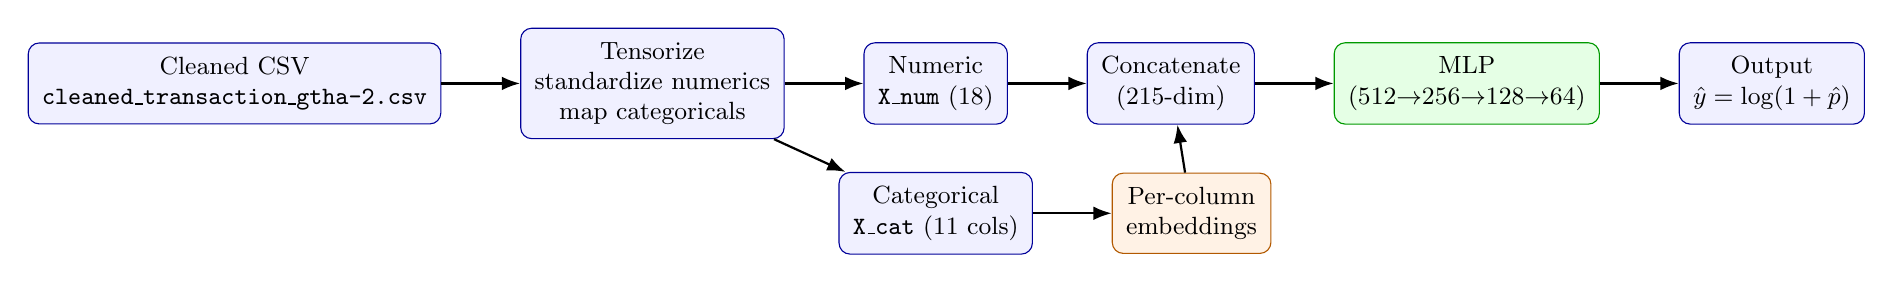
\begin{tikzpicture}[
  node/.style={draw, rounded corners, align=center, inner sep=5pt, font=\small},
  arrow/.style={-Latex, thick},
  box/.style={node, fill=blue!6, draw=blue!60!black},
  emb/.style={node, fill=orange!10, draw=orange!70!black},
  mlp/.style={node, fill=green!10, draw=green!60!black},
]
\node[box] (csv) {Cleaned CSV\\\texttt{cleaned\_transaction\_gtha-2.csv}};
\node[box, right=10mm of csv] (ten) {Tensorize\\standardize numerics\\map categoricals};
\node[box, right=10mm of ten] (num) {Numeric\\\texttt{X\_num} (18)};
\node[box, below=6mm of num] (cat) {Categorical\\\texttt{X\_cat} (11 cols)};
\node[emb, right=10mm of cat] (embs) {Per-column\\embeddings};
\node[box, right=10mm of num] (concat) {Concatenate\\(215-dim)};
\node[mlp, right=10mm of concat] (mlp) {MLP\\(512$\to$256$\to$128$\to$64)};
\node[box, right=10mm of mlp] (out) {Output\\\(\hat{y}=\log(1+\hat{p})\)};
\draw[arrow] (csv) -- (ten);
\draw[arrow] (ten) -- (num);
\draw[arrow] (ten) -- (cat);
\draw[arrow] (num) -- (concat);
\draw[arrow] (cat) -- (embs);
\draw[arrow] (embs) -- (concat);
\draw[arrow] (concat) -- (mlp);
\draw[arrow] (mlp) -- (out);
\end{tikzpicture}
\caption{End-to-end pipeline illustration (same core idea as the main report).}
\label{fig:appendix-pipeline}
\end{figure}

\begin{figure}[t]
\centering
\begin{subfigure}{0.49\linewidth}
\centering
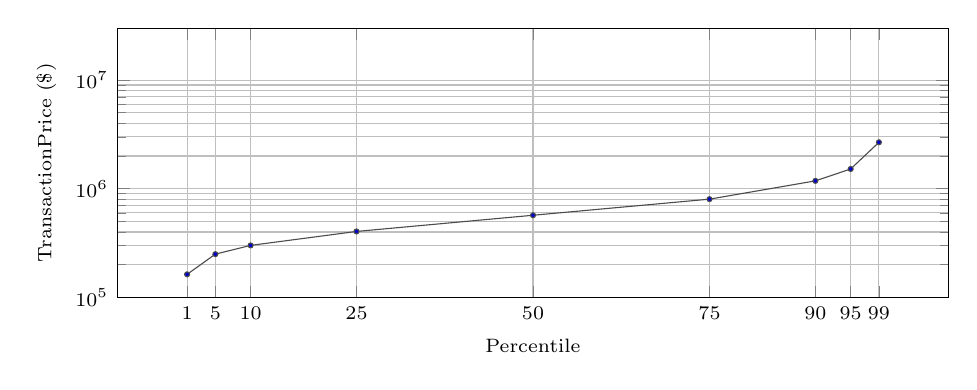
\begin{tikzpicture}
\begin{axis}[
  width=\linewidth,
  height=5.0cm,
  xlabel={Percentile},
  ylabel={TransactionPrice (\$)},
  ymode=log,
  log basis y=10,
  ymin=1e5, ymax=3e7,
  xtick={1,5,10,25,50,75,90,95,99},
  grid=both,
  tick label style={font=\scriptsize},
  label style={font=\scriptsize},
]
\addplot+[mark=*, mark size=0.9pt, color=black!70] coordinates {
  (1,163000)
  (5,250000)
  (10,301000)
  (25,404486)
  (50,570000)
  (75,801800)
  (90,1181000)
  (95,1520000)
  (99,2675365)
};
\end{axis}
\end{tikzpicture}
\caption{Price distribution (selected percentiles; log y-axis).}
\label{fig:appendix-price-dist}
\end{subfigure}
\hfill
\begin{subfigure}{0.49\linewidth}
\centering
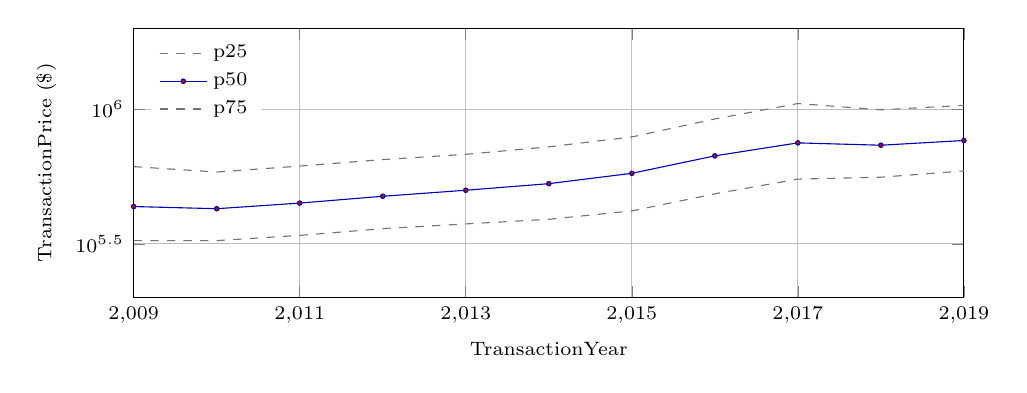
\begin{tikzpicture}
\begin{axis}[
  width=\linewidth,
  height=5.0cm,
  xlabel={TransactionYear},
  ylabel={TransactionPrice (\$)},
  ymode=log,
  log basis y=10,
  xmin=2009, xmax=2019,
  xtick={2009,2011,2013,2015,2017,2019},
  ymin=2e5, ymax=2e6,
  grid=both,
  tick label style={font=\scriptsize},
  label style={font=\scriptsize},
  legend style={font=\scriptsize, at={(0.02,0.98)}, anchor=north west, draw=none},
]
\addplot+[mark=none, dashed, color=black!55] coordinates {
  (2009,325000) (2010,325000) (2011,339900) (2012,360000) (2013,375000) (2014,390000) (2015,419000) (2016,485000) (2017,550000) (2018,559000) (2019,590000)
};
\addlegendentry{p25}
\addplot+[mark=*, mark size=0.8pt, color=blue!70!black] coordinates {
  (2009,435000) (2010,427000) (2011,448000) (2012,475000) (2013,500000) (2014,529000) (2015,578000) (2016,671100) (2017,750000) (2018,735000) (2019,765500)
};
\addlegendentry{p50}
\addplot+[mark=none, dashed, color=black!55] coordinates {
  (2009,612000) (2010,584300) (2011,615000) (2012,650000) (2013,680000) (2014,725000) (2015,789000) (2016,920000) (2017,1050000) (2018,995000) (2019,1033625)
};
\addlegendentry{p75}
\end{axis}
\end{tikzpicture}
\caption{Non-stationarity (2009--2019): yearly p25/p50/p75 (log y-axis).}
\label{fig:appendix-market-drift}
\end{subfigure}
\caption{Dataset context plots.}
\label{fig:appendix-dataset}
\end{figure}

\clearpage
\section{Quantitative results (comparisons)}

\begin{table}[t]
\centering
\small
\setlength{\tabcolsep}{4pt}
\begin{tabular}{@{}lrrrrr@{}}
\toprule
Model & Params & Rand RMSE & Rand Acc(\%) & Time RMSE & Time Acc(\%) \\
\midrule
Constant (mean) & 0 & \NaiveMeanRmse & \NaiveMeanAcc & -- & -- \\
Hedonic & 7{,}254 & \HedRandRmseMean\(\pm\)\HedRandRmseStd & \HedRandAccMean\(\pm\)\HedRandAccStd & \HedTimeRmseMean\(\pm\)\HedTimeRmseStd & \HedTimeAccMean\(\pm\)\HedTimeAccStd \\
FM (2-way) & \FmParams & \FmTestRmse & \FmTestAcc & \FmTimeTestRmse & \FmTimeTestAcc \\
TabNet & \TabnetParams & \TabnetTestRmse & \TabnetTestAcc & \TabnetTimeTestRmse & \TabnetTimeTestAcc \\
TabTransformer & \TabtrParams & \TabtrTestRmse & \TabtrTestAcc & \TabtrTimeTestRmse & \TabtrTimeTestAcc \\
FT-Transformer & \FtParams & \FtTestRmse & \FtTestAcc & \FtTimeTestRmse & \FtTimeTestAcc \\
DeepFM & 3{,}146{,}151 & \DeepRandRmseMean\(\pm\)\DeepRandRmseStd & \DeepRandAccMean\(\pm\)\DeepRandAccStd & \DeepTimeRmseMean\(\pm\)\DeepTimeRmseStd & \DeepTimeAccMean\(\pm\)\DeepTimeAccStd \\
ANN (embed+MLP) & \AnnParams & \AnnRandRmseMean\(\pm\)\AnnRandRmseStd & \AnnRandAccMean\(\pm\)\AnnRandAccStd & \AnnTimeRmseMean\(\pm\)\AnnTimeRmseStd & \AnnTimeAccMean\(\pm\)\AnnTimeAccStd \\
\bottomrule
\end{tabular}
\caption{All-model quantitative summary (same numbers as the main report; RMSE is in log space).}
\label{tab:appendix-all-models}
\end{table}

\begin{figure}[t]
\centering
\begin{subfigure}{0.49\linewidth}
\centering
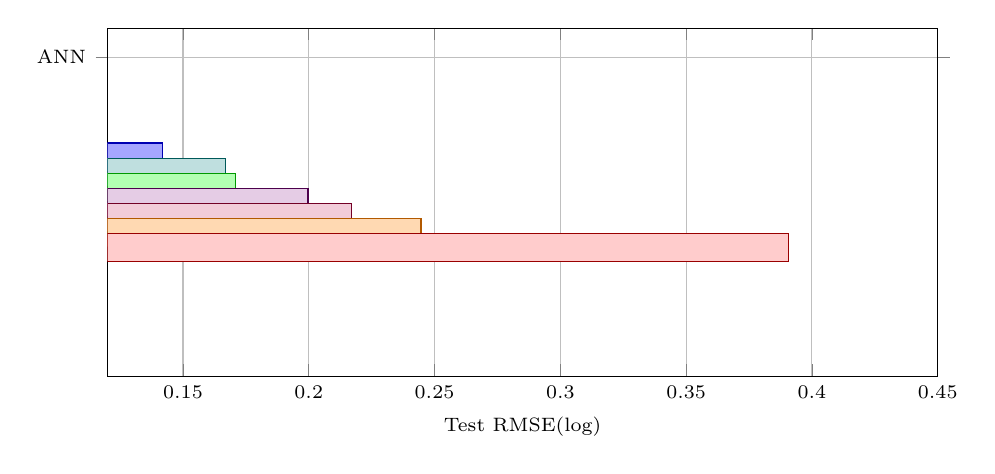
\begin{tikzpicture}
\begin{axis}[
  xbar,
  width=\linewidth,
  height=6.0cm,
  xlabel={Test RMSE(log)},
  symbolic y coords={ANN,FT-Transformer,DeepFM,TabTransformer,FM,Hedonic,TabNet},
  ytick=data,
  y dir=reverse,
  xmin=0.12, xmax=0.45,
  grid=both,
  tick label style={font=\scriptsize},
  label style={font=\scriptsize},
]
\addplot+[fill=blue!35, draw=blue!70!black] coordinates {(\AnnRandRmseMean,ANN)};
\addplot+[fill=teal!25, draw=teal!70!black] coordinates {(\FtTestRmse,FT-Transformer)};
\addplot+[fill=green!30, draw=green!60!black] coordinates {(\DeepRandRmseMean,DeepFM)};
\addplot+[fill=violet!20, draw=violet!60!black] coordinates {(\TabtrTestRmse,TabTransformer)};
\addplot+[fill=purple!20, draw=purple!60!black] coordinates {(\FmTestRmse,FM)};
\addplot+[fill=orange!30, draw=orange!70!black] coordinates {(\HedRandRmseMean,Hedonic)};
\addplot+[fill=red!20, draw=red!60!black] coordinates {(\TabnetTestRmse,TabNet)};
\end{axis}
\end{tikzpicture}
\caption{Random split RMSE(log).}
\label{fig:appendix-allmodels-rand-rmse}
\end{subfigure}
\hfill
\begin{subfigure}{0.49\linewidth}
\centering
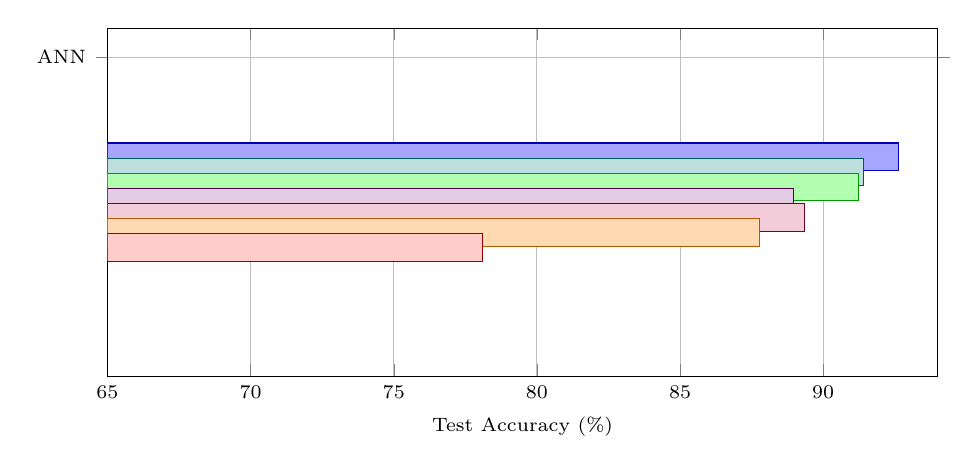
\begin{tikzpicture}
\begin{axis}[
  xbar,
  width=\linewidth,
  height=6.0cm,
  xlabel={Test Accuracy (\%)},
  symbolic y coords={ANN,FT-Transformer,DeepFM,TabTransformer,FM,Hedonic,TabNet},
  ytick=data,
  y dir=reverse,
  xmin=65, xmax=94,
  grid=both,
  tick label style={font=\scriptsize},
  label style={font=\scriptsize},
]
\addplot+[fill=blue!35, draw=blue!70!black] coordinates {(\AnnRandAccMean,ANN)};
\addplot+[fill=teal!25, draw=teal!70!black] coordinates {(\FtTestAcc,FT-Transformer)};
\addplot+[fill=green!30, draw=green!60!black] coordinates {(\DeepRandAccMean,DeepFM)};
\addplot+[fill=violet!20, draw=violet!60!black] coordinates {(\TabtrTestAcc,TabTransformer)};
\addplot+[fill=purple!20, draw=purple!60!black] coordinates {(\FmTestAcc,FM)};
\addplot+[fill=orange!30, draw=orange!70!black] coordinates {(\HedRandAccMean,Hedonic)};
\addplot+[fill=red!20, draw=red!60!black] coordinates {(\TabnetTestAcc,TabNet)};
\end{axis}
\end{tikzpicture}
\caption{Random split accuracy.}
\label{fig:appendix-allmodels-rand-acc}
\end{subfigure}

\vspace{1mm}

\begin{subfigure}{0.49\linewidth}
\centering
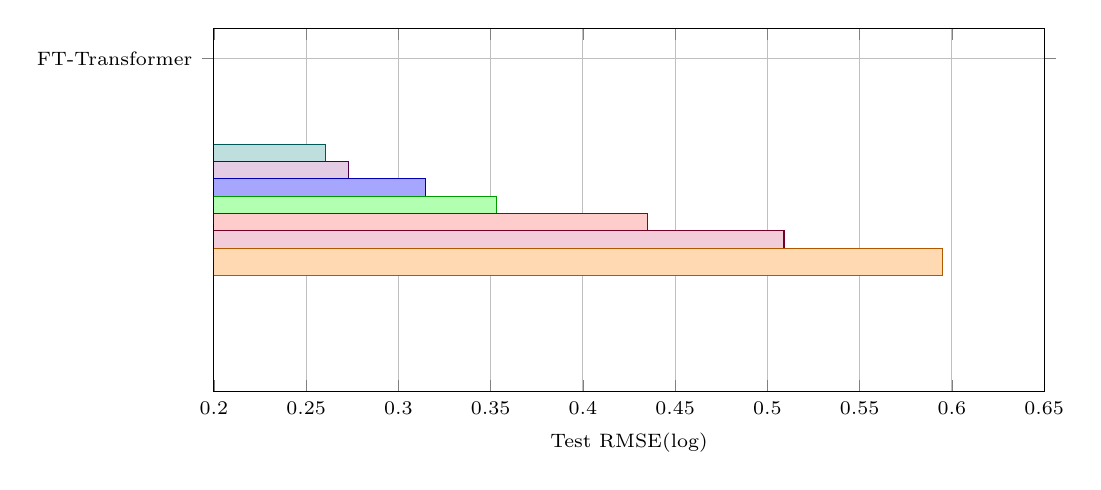
\begin{tikzpicture}
\begin{axis}[
  xbar,
  width=\linewidth,
  height=6.2cm,
  xlabel={Test RMSE(log)},
  symbolic y coords={FT-Transformer,TabTransformer,ANN,DeepFM,TabNet,FM,Hedonic},
  ytick=data,
  y dir=reverse,
  xmin=0.20, xmax=0.65,
  grid=both,
  tick label style={font=\scriptsize},
  label style={font=\scriptsize},
]
\addplot+[fill=teal!25, draw=teal!70!black] coordinates {(\FtTimeTestRmse,FT-Transformer)};
\addplot+[fill=violet!20, draw=violet!60!black] coordinates {(\TabtrTimeTestRmse,TabTransformer)};
\addplot+[fill=blue!35, draw=blue!70!black] coordinates {(\AnnTimeRmseMean,ANN)};
\addplot+[fill=green!30, draw=green!60!black] coordinates {(\DeepTimeRmseMean,DeepFM)};
\addplot+[fill=red!20, draw=red!60!black] coordinates {(\TabnetTimeTestRmse,TabNet)};
\addplot+[fill=purple!20, draw=purple!60!black] coordinates {(\FmTimeTestRmse,FM)};
\addplot+[fill=orange!30, draw=orange!70!black] coordinates {(\HedTimeRmseMean,Hedonic)};
\end{axis}
\end{tikzpicture}
\caption{Time split RMSE(log).}
\label{fig:appendix-allmodels-time-rmse}
\end{subfigure}
\hfill
\begin{subfigure}{0.49\linewidth}
\centering
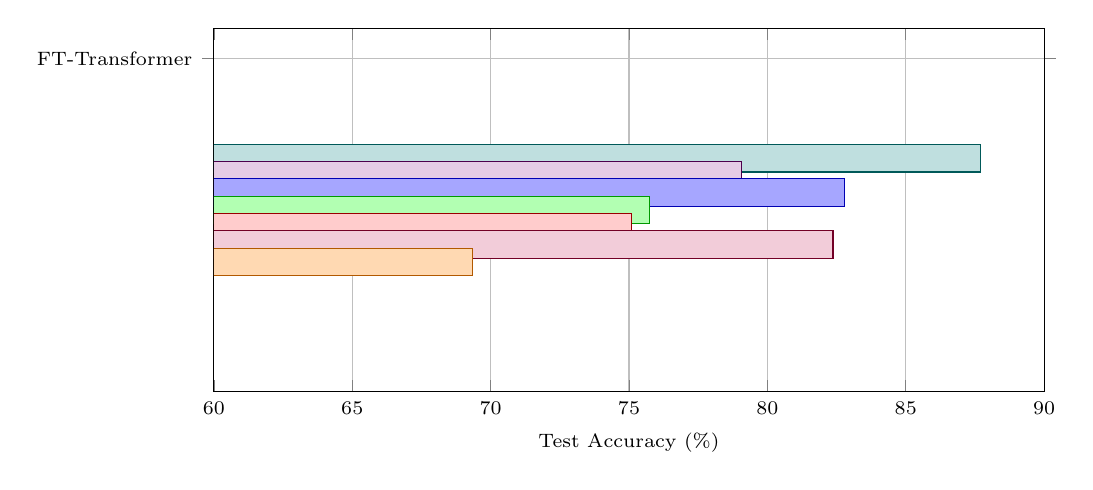
\begin{tikzpicture}
\begin{axis}[
  xbar,
  width=\linewidth,
  height=6.2cm,
  xlabel={Test Accuracy (\%)},
  symbolic y coords={FT-Transformer,TabTransformer,ANN,DeepFM,TabNet,FM,Hedonic},
  ytick=data,
  y dir=reverse,
  xmin=60, xmax=90,
  grid=both,
  tick label style={font=\scriptsize},
  label style={font=\scriptsize},
]
\addplot+[fill=teal!25, draw=teal!70!black] coordinates {(\FtTimeTestAcc,FT-Transformer)};
\addplot+[fill=violet!20, draw=violet!60!black] coordinates {(\TabtrTimeTestAcc,TabTransformer)};
\addplot+[fill=blue!35, draw=blue!70!black] coordinates {(\AnnTimeAccMean,ANN)};
\addplot+[fill=green!30, draw=green!60!black] coordinates {(\DeepTimeAccMean,DeepFM)};
\addplot+[fill=red!20, draw=red!60!black] coordinates {(\TabnetTimeTestAcc,TabNet)};
\addplot+[fill=purple!20, draw=purple!60!black] coordinates {(\FmTimeTestAcc,FM)};
\addplot+[fill=orange!30, draw=orange!70!black] coordinates {(\HedTimeAccMean,Hedonic)};
\end{axis}
\end{tikzpicture}
\caption{Time split accuracy.}
\label{fig:appendix-allmodels-time-acc}
\end{subfigure}

\caption{All-model bar charts (mix of robustness means and single full-train runs; see Table~\ref{tab:appendix-all-models}).}
\label{fig:appendix-allmodels-bars}
\end{figure}

\begin{figure}[t]
\centering
\begin{subfigure}{0.49\linewidth}
\centering
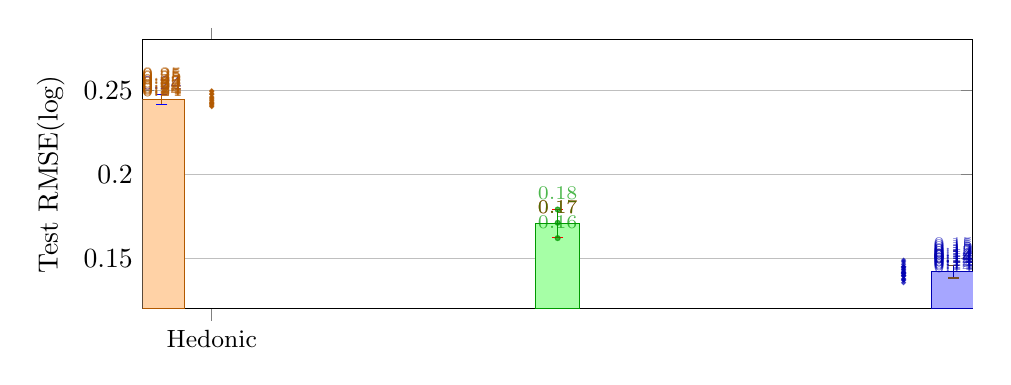
\begin{tikzpicture}
\begin{axis}[
  ybar,
  width=\linewidth,
  height=5.0cm,
  bar width=16pt,
  ylabel={Test RMSE(log)},
  symbolic x coords={Hedonic,DeepFM,ANN},
  xtick=data,
  ymin=0.12, ymax=0.28,
  ymajorgrids=true,
  error bars/y dir=both,
  error bars/y explicit,
  nodes near coords,
  every node near coord/.append style={font=\scriptsize},
  xticklabel style={font=\small},
]
\addplot+[fill=orange!35, draw=orange!70!black] coordinates {(Hedonic,\HedRandRmseMean) +- (0,\HedRandRmseStd)};
\addplot+[fill=green!35, draw=green!60!black] coordinates {(DeepFM,\DeepRandRmseMean) +- (0,\DeepRandRmseStd)};
\addplot+[fill=blue!35, draw=blue!70!black] coordinates {(ANN,\AnnRandRmseMean) +- (0,\AnnRandRmseStd)};
\addplot+[only marks, mark=*, mark size=0.7pt, color=orange!70!black, opacity=0.6] coordinates {
  (Hedonic,0.2426) (Hedonic,0.2402) (Hedonic,0.2497) (Hedonic,0.2480) (Hedonic,0.2476) (Hedonic,0.2439) (Hedonic,0.2424) (Hedonic,0.2408) (Hedonic,0.2422) (Hedonic,0.2494) (Hedonic,0.2475) (Hedonic,0.2491) (Hedonic,0.2459) (Hedonic,0.2441) (Hedonic,0.2459) (Hedonic,0.2452) (Hedonic,0.2431) (Hedonic,0.2447) (Hedonic,0.2419) (Hedonic,0.2405) (Hedonic,0.2416)
};
\addplot+[only marks, mark=*, mark size=0.9pt, color=green!60!black, opacity=0.7] coordinates {
  (DeepFM,0.1791) (DeepFM,0.1712) (DeepFM,0.1621)
};
\addplot+[only marks, mark=*, mark size=0.7pt, color=blue!70!black, opacity=0.6] coordinates {
  (ANN,0.1434) (ANN,0.1399) (ANN,0.1375) (ANN,0.1466) (ANN,0.1370) (ANN,0.1409) (ANN,0.1447) (ANN,0.1452) (ANN,0.1480) (ANN,0.1438) (ANN,0.1356) (ANN,0.1409) (ANN,0.1490) (ANN,0.1396) (ANN,0.1418) (ANN,0.1397) (ANN,0.1380) (ANN,0.1426) (ANN,0.1416) (ANN,0.1414) (ANN,0.1450)
};
\end{axis}
\end{tikzpicture}
\caption{Random split RMSE (mean \(\pm\) std; ANN/Hedonic \(n=21\), DeepFM \(n=3\)).}
\end{subfigure}
\hfill
\begin{subfigure}{0.49\linewidth}
\centering
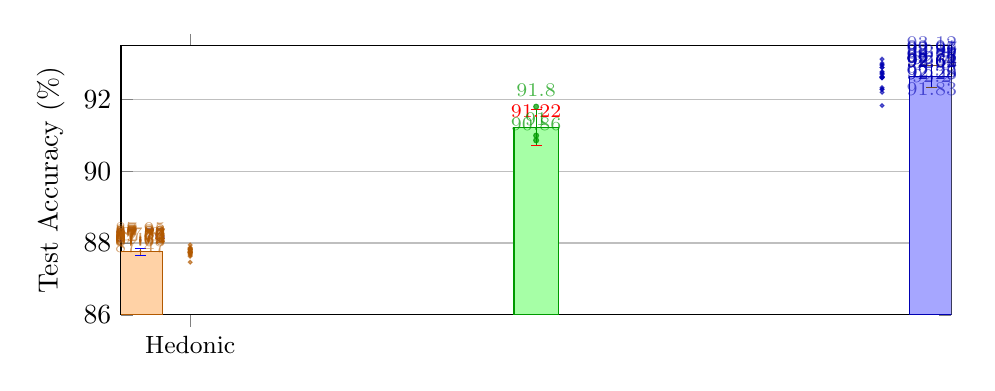
\begin{tikzpicture}
\begin{axis}[
  ybar,
  width=\linewidth,
  height=5.0cm,
  bar width=16pt,
  ylabel={Test Accuracy (\%)},
  symbolic x coords={Hedonic,DeepFM,ANN},
  xtick=data,
  ymin=86, ymax=93.5,
  ymajorgrids=true,
  error bars/y dir=both,
  error bars/y explicit,
  nodes near coords,
  every node near coord/.append style={font=\scriptsize},
  xticklabel style={font=\small},
]
\addplot+[fill=orange!35, draw=orange!70!black] coordinates {(Hedonic,\HedRandAccMean) +- (0,\HedRandAccStd)};
\addplot+[fill=green!35, draw=green!60!black] coordinates {(DeepFM,\DeepRandAccMean) +- (0,\DeepRandAccStd)};
\addplot+[fill=blue!35, draw=blue!70!black] coordinates {(ANN,\AnnRandAccMean) +- (0,\AnnRandAccStd)};
\addplot+[only marks, mark=*, mark size=0.7pt, color=orange!70!black, opacity=0.6] coordinates {
  (Hedonic,87.7199) (Hedonic,87.9470) (Hedonic,87.8302) (Hedonic,87.8754) (Hedonic,87.4666) (Hedonic,87.6624) (Hedonic,87.7216) (Hedonic,87.7659) (Hedonic,87.7390) (Hedonic,87.7773) (Hedonic,87.8040) (Hedonic,87.7355) (Hedonic,87.7418) (Hedonic,87.8550) (Hedonic,87.6301) (Hedonic,87.7703) (Hedonic,87.8154) (Hedonic,87.7429) (Hedonic,87.8378) (Hedonic,87.6905) (Hedonic,87.8113)
};
\addplot+[only marks, mark=*, mark size=0.9pt, color=green!60!black, opacity=0.7] coordinates {
  (DeepFM,90.9951) (DeepFM,90.8615) (DeepFM,91.8002)
};
\addplot+[only marks, mark=*, mark size=0.7pt, color=blue!70!black, opacity=0.6] coordinates {
  (ANN,92.7739) (ANN,92.9570) (ANN,93.0117) (ANN,92.2799) (ANN,92.9697) (ANN,92.6272) (ANN,92.7600) (ANN,92.6082) (ANN,92.3316) (ANN,92.2886) (ANN,92.8901) (ANN,92.6005) (ANN,91.8307) (ANN,92.7244) (ANN,92.6367) (ANN,92.8954) (ANN,93.1237) (ANN,92.6203) (ANN,92.6233) (ANN,92.7038) (ANN,92.2001)
};
\end{axis}
\end{tikzpicture}
\caption{Random split accuracy (mean \(\pm\) std; ANN/Hedonic \(n=21\), DeepFM \(n=3\)).}
\end{subfigure}

\vspace{1mm}

\begin{subfigure}{0.49\linewidth}
\centering
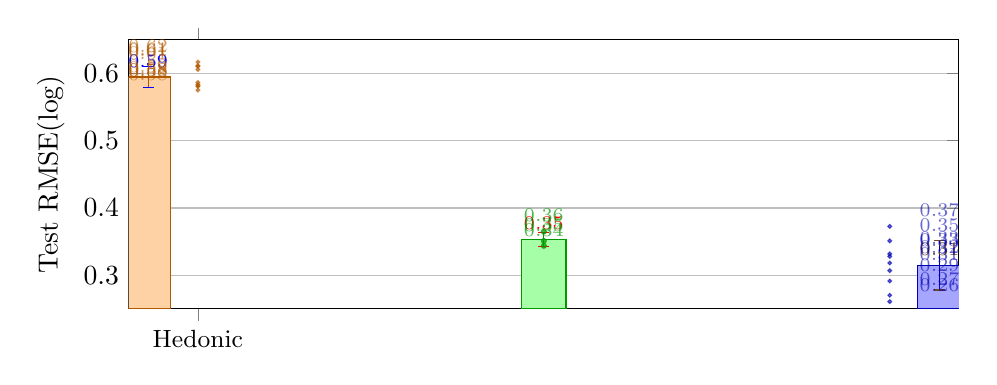
\begin{tikzpicture}
\begin{axis}[
  ybar,
  width=\linewidth,
  height=5.0cm,
  bar width=16pt,
  ylabel={Test RMSE(log)},
  symbolic x coords={Hedonic,DeepFM,ANN},
  xtick=data,
  ymin=0.25, ymax=0.65,
  ymajorgrids=true,
  error bars/y dir=both,
  error bars/y explicit,
  nodes near coords,
  every node near coord/.append style={font=\scriptsize},
  xticklabel style={font=\small},
]
\addplot+[fill=orange!35, draw=orange!70!black] coordinates {(Hedonic,\HedTimeRmseMean) +- (0,\HedTimeRmseStd)};
\addplot+[fill=green!35, draw=green!60!black] coordinates {(DeepFM,\DeepTimeRmseMean) +- (0,\DeepTimeRmseStd)};
\addplot+[fill=blue!35, draw=blue!70!black] coordinates {(ANN,\AnnTimeRmseMean) +- (0,\AnnTimeRmseStd)};
\addplot+[only marks, mark=*, mark size=0.7pt, color=orange!70!black, opacity=0.6] coordinates {
  (Hedonic,0.6106) (Hedonic,0.5808) (Hedonic,0.6059) (Hedonic,0.5864) (Hedonic,0.6114) (Hedonic,0.5815) (Hedonic,0.6168) (Hedonic,0.5752) (Hedonic,0.5833)
};
\addplot+[only marks, mark=*, mark size=0.9pt, color=green!60!black, opacity=0.7] coordinates {
  (DeepFM,0.3438) (DeepFM,0.3511) (DeepFM,0.3649)
};
\addplot+[only marks, mark=*, mark size=0.7pt, color=blue!70!black, opacity=0.6] coordinates {
  (ANN,0.3319) (ANN,0.3511) (ANN,0.3727) (ANN,0.3068) (ANN,0.2915) (ANN,0.2609) (ANN,0.3281) (ANN,0.3183) (ANN,0.2703)
};
\end{axis}
\end{tikzpicture}
\caption{Time split RMSE (mean \(\pm\) std; ANN/Hedonic \(n=9\), DeepFM \(n=3\)).}
\end{subfigure}
\hfill
\begin{subfigure}{0.49\linewidth}
\centering
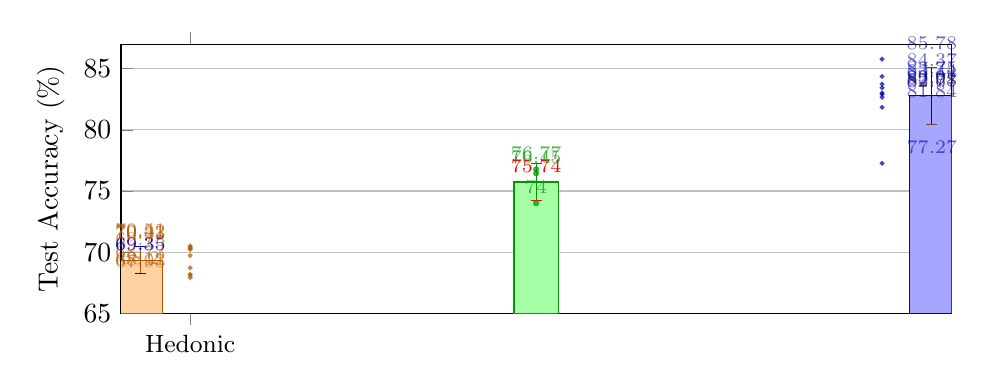
\begin{tikzpicture}
\begin{axis}[
  ybar,
  width=\linewidth,
  height=5.0cm,
  bar width=16pt,
  ylabel={Test Accuracy (\%)},
  symbolic x coords={Hedonic,DeepFM,ANN},
  xtick=data,
  ymin=65, ymax=87,
  ymajorgrids=true,
  error bars/y dir=both,
  error bars/y explicit,
  nodes near coords,
  every node near coord/.append style={font=\scriptsize},
  xticklabel style={font=\small},
]
\addplot+[fill=orange!35, draw=orange!70!black] coordinates {(Hedonic,\HedTimeAccMean) +- (0,\HedTimeAccStd)};
\addplot+[fill=green!35, draw=green!60!black] coordinates {(DeepFM,\DeepTimeAccMean) +- (0,\DeepTimeAccStd)};
\addplot+[fill=blue!35, draw=blue!70!black] coordinates {(ANN,\AnnTimeAccMean) +- (0,\AnnTimeAccStd)};
\addplot+[only marks, mark=*, mark size=0.7pt, color=orange!70!black, opacity=0.6] coordinates {
  (Hedonic,68.2017) (Hedonic,70.2305) (Hedonic,68.7268) (Hedonic,69.7324) (Hedonic,68.1137) (Hedonic,70.5108) (Hedonic,67.9282) (Hedonic,70.4157) (Hedonic,70.3063)
};
\addplot+[only marks, mark=*, mark size=0.9pt, color=green!60!black, opacity=0.7] coordinates {
  (DeepFM,76.4491) (DeepFM,76.7739) (DeepFM,74.0039)
};
\addplot+[only marks, mark=*, mark size=0.7pt, color=blue!70!black, opacity=0.6] coordinates {
  (ANN,81.8443) (ANN,82.9056) (ANN,77.2688) (ANN,83.0138) (ANN,83.7456) (ANN,85.7801) (ANN,82.6667) (ANN,83.4415) (ANN,84.3658)
};
\end{axis}
\end{tikzpicture}
\caption{Time split accuracy (mean \(\pm\) std; ANN/Hedonic \(n=9\), DeepFM \(n=3\)).}
\end{subfigure}

\vspace{-1mm}
\caption{Robustness-style comparisons with error bars and per-run dots (ANN vs hedonic baseline vs DeepFM).}
\label{fig:appendix-robustness}
\end{figure}

\clearpage
\section{Qualitative diagnostics (ANN)}
\ifannqual

\begin{figure}[t]
\centering
\begin{subfigure}{0.49\linewidth}
\centering
\begin{tikzpicture}
\begin{axis}[
  width=\linewidth,
  height=5.0cm,
  xlabel={True \(\log(1+\text{price})\)},
  ylabel={Pred \(\log(1+\text{price})\)},
  xmin=11.0, xmax=16.0,
  ymin=11.0, ymax=16.0,
  grid=both,
  tick label style={font=\scriptsize},
  label style={font=\scriptsize},
  legend style={font=\scriptsize, at={(0.02,0.98)}, anchor=north west, draw=none},
]
\addplot+[only marks, mark=o, mark size=1.2pt, color=blue!70!black, opacity=0.55] table[x=true,y=pred] {\AnnPredScatter};
\addlegendentry{ANN samples}
\addplot+[domain=11:16, samples=2, color=black!60] {x};
\addlegendentry{Ideal y=x}
\end{axis}
\end{tikzpicture}
\caption{Predicted vs true (sampled).}
\label{fig:appendix-ann-scatter}
\end{subfigure}
\hfill
\begin{subfigure}{0.49\linewidth}
\centering
\begin{tikzpicture}
\begin{axis}[
  ybar,
  width=\linewidth,
  height=5.0cm,
  bar width=5pt,
  xlabel={Residual (pred$-$true) in \(\log(1+\text{price})\)},
  ylabel={Count},
  xmin=-1.05, xmax=1.05,
  ymajorgrids=true,
  tick label style={font=\scriptsize},
  label style={font=\scriptsize},
]
\addplot+[fill=blue!18, draw=blue!60!black] table[x=center,y=count] {\AnnResidHist};
\end{axis}
\end{tikzpicture}
\caption{Residual histogram (full test).}
\label{fig:appendix-ann-resid}
\end{subfigure}

\vspace{1mm}

\begin{subfigure}{0.49\linewidth}
\centering
\begin{tikzpicture}
\begin{axis}[
  width=\linewidth,
  height=4.2cm,
  xlabel={True-price decile (1=lowest, 10=highest)},
  ylabel={Accuracy (\%)},
  xmin=1, xmax=10,
  ymin=86, ymax=95,
  xtick={1,2,3,4,5,6,7,8,9,10},
  grid=both,
  tick label style={font=\scriptsize},
  label style={font=\scriptsize},
]
\addplot+[mark=*, mark size=1.4pt, color=purple!70!black] table[x=decile,y=acc] {\AnnByPriceDecile};
\end{axis}
\end{tikzpicture}
\caption{Accuracy by true-price decile.}
\label{fig:appendix-ann-decile-acc}
\end{subfigure}
\hfill
\begin{subfigure}{0.49\linewidth}
\centering
\begin{tikzpicture}
\begin{axis}[
  width=\linewidth,
  height=4.2cm,
  xlabel={True-price decile (1=lowest, 10=highest)},
  ylabel={MdAPE (\%)},
  xmin=1, xmax=10,
  ymin=5, ymax=13,
  xtick={1,2,3,4,5,6,7,8,9,10},
  grid=both,
  tick label style={font=\scriptsize},
  label style={font=\scriptsize},
]
\addplot+[mark=triangle*, mark size=1.4pt, color=red!70!black] table[x=decile,y expr=\thisrow{mdape}*100] {\AnnByPriceDecile};
\end{axis}
\end{tikzpicture}
\caption{MdAPE by true-price decile.}
\label{fig:appendix-ann-decile-mdape}
\end{subfigure}

\caption{ANN qualitative diagnostics (random split, seed=42). APE percentiles: median \AnnApeP50\%, p90 \AnnApeP90\%, p95 \AnnApeP95\%, p99 \AnnApeP99\%.}
\label{fig:appendix-ann-qual}
\end{figure}

\begin{figure}[t]
\centering
\begin{subfigure}{0.49\linewidth}
\centering
\begin{tikzpicture}
\begin{axis}[
  ybar,
  width=\linewidth,
  height=5.0cm,
  xlabel={TransactionYear},
  ylabel={Accuracy (\%)},
  symbolic x coords={2009,2010,2011,2012,2013,2014,2015,2016,2017,2018,2019},
  xtick=data,
  x tick label style={rotate=45,anchor=east},
  ymin=90, ymax=94,
  ymajorgrids=true,
  tick label style={font=\scriptsize},
  label style={font=\scriptsize},
]
\addplot+[fill=green!18, draw=green!60!black] table[x=year,y=acc] {\AnnByYear};
\end{axis}
\end{tikzpicture}
\caption{Accuracy by year (2009--2019 subset).}
\label{fig:appendix-ann-year-acc}
\end{subfigure}
\hfill
\begin{subfigure}{0.49\linewidth}
\centering
\begin{tikzpicture}
\begin{axis}[
  ybar,
  width=\linewidth,
  height=5.0cm,
  xlabel={TransactionYear},
  ylabel={MdAPE (\%)},
  symbolic x coords={2009,2010,2011,2012,2013,2014,2015,2016,2017,2018,2019},
  xtick=data,
  x tick label style={rotate=45,anchor=east},
  ymin=5, ymax=10,
  ymajorgrids=true,
  tick label style={font=\scriptsize},
  label style={font=\scriptsize},
]
\addplot+[fill=orange!22, draw=orange!70!black] table[x=year,y expr=\thisrow{mdape}*100] {\AnnByYear};
\end{axis}
\end{tikzpicture}
\caption{MdAPE by year (2009--2019 subset).}
\label{fig:appendix-ann-year-mdape}
\end{subfigure}
\caption{ANN performance segmentation by transaction year (random-split test set).}
\label{fig:appendix-ann-year}
\end{figure}

\else
\textbf{Missing \texttt{ann\_qual\_data.tex}.} Generate it with:
\begin{quote}
\texttt{python make\_ann\_qual\_data.py --data ann\_tensors\_full.pt}
\end{quote}
\fi

\clearpage
\section{Analysis / interpretability}

\begin{figure}[t]
\centering
\begin{subfigure}{0.32\linewidth}
\centering
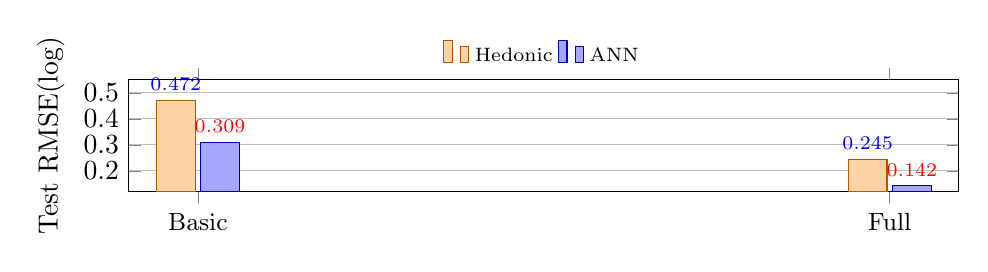
\begin{tikzpicture}
\begin{axis}[
  ybar,
  width=\linewidth,
  height=3.0cm,
  bar width=14pt,
  ylabel={Test RMSE(log)},
  symbolic x coords={Basic,Full},
  xtick=data,
  ymin=0.12, ymax=0.55,
  ymajorgrids=true,
  nodes near coords,
  nodes near coords style={/pgf/number format/fixed, /pgf/number format/precision=3},
  every node near coord/.append style={font=\scriptsize},
  xticklabel style={font=\small},
  legend style={font=\scriptsize, at={(0.5,1.02)}, anchor=south, legend columns=2, draw=none},
]
\addplot+[fill=orange!35, draw=orange!70!black] coordinates {(Basic,\BasicHedTestRmse) (Full,\HedRandRmseMean)};
\addplot+[fill=blue!35, draw=blue!70!black] coordinates {(Basic,\BasicAnnTestRmse) (Full,\AnnRandRmseMean)};
\legend{Hedonic,ANN}
\end{axis}
\end{tikzpicture}
\caption{Feature-set ablation (seed=42): \texttt{basic} vs \texttt{full}.}
\label{fig:appendix-ablation}
\end{subfigure}
\hfill
\begin{subfigure}{0.32\linewidth}
\centering
\begin{tikzpicture}
\begin{axis}[
  xbar,
  width=\linewidth,
  height=3.0cm,
  xlabel={Δ validation MSE},
  ytick=data,
  y dir=reverse,
  yticklabels={LivingArea,TransactionYear,FSA,gcode\_City,YearBuilt,BuildingType,Ownership,PropertyStyle},
  xmin=0, xmax=0.11,
  grid=both,
  tick label style={font=\scriptsize},
  label style={font=\scriptsize},
]
\addplot+[fill=blue!25, draw=blue!60!black] coordinates {
  (0.098610,0) (0.089895,1) (0.066793,2) (0.042350,3)
  (0.011641,4) (0.009254,5) (0.007690,6) (0.006414,7)
};
\end{axis}
\end{tikzpicture}
\caption{Permutation importance (ANN; 20k-row val subset).}
\label{fig:appendix-perm}
\end{subfigure}
\hfill
\begin{subfigure}{0.32\linewidth}
\centering
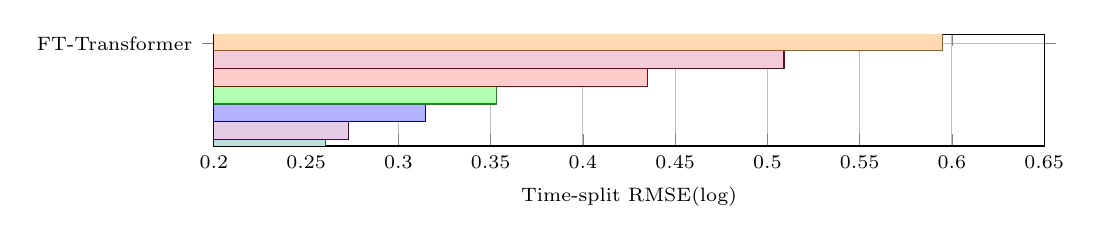
\begin{tikzpicture}
\begin{axis}[
  xbar,
  width=\linewidth,
  height=3.0cm,
  xlabel={Time-split RMSE(log)},
  symbolic y coords={FT-Transformer,TabTransformer,ANN,DeepFM,TabNet,FM,Hedonic},
  ytick=data,
  y dir=reverse,
  xmin=0.20, xmax=0.65,
  grid=both,
  tick label style={font=\scriptsize},
  label style={font=\scriptsize},
]
\addplot+[fill=teal!25, draw=teal!70!black] coordinates {(\FtTimeTestRmse,FT-Transformer)};
\addplot+[fill=violet!20, draw=violet!60!black] coordinates {(\TabtrTimeTestRmse,TabTransformer)};
\addplot+[fill=blue!30, draw=blue!70!black] coordinates {(\AnnTimeRmseMean,ANN)};
\addplot+[fill=green!30, draw=green!60!black] coordinates {(\DeepTimeRmseMean,DeepFM)};
\addplot+[fill=red!20, draw=red!60!black] coordinates {(\TabnetTimeTestRmse,TabNet)};
\addplot+[fill=purple!20, draw=purple!60!black] coordinates {(\FmTimeTestRmse,FM)};
\addplot+[fill=orange!30, draw=orange!70!black] coordinates {(\HedTimeRmseMean,Hedonic)};
\end{axis}
\end{tikzpicture}
\caption{Time split model ranking (RMSE).}
\label{fig:appendix-time-ranking}
\end{subfigure}
\caption{Analysis/interpretability visuals.}
\label{fig:appendix-analysis}
\end{figure}

\begin{figure}[t]
\centering
\begin{tikzpicture}
\begin{axis}[
  width=\linewidth,
  height=7.0cm,
  xlabel={Train time per run (minutes; CPU)},
  ylabel={Interpretability score (1=low, 5=high)},
  xmin=0, xmax=22,
  ymin=0.5, ymax=5.5,
  ytick={1,2,3,4,5},
  grid=both,
  tick label style={font=\scriptsize},
  label style={font=\scriptsize},
  nodes near coords,
  point meta=explicit symbolic,
  every node near coord/.append style={font=\scriptsize, anchor=west, xshift=2pt},
]
\addplot+[
  only marks,
  mark=*,
  mark size=2.2pt,
  color=blue!70!black,
] table[x=minutes,y=interp,meta=label] {\TrainTimeInterp};
\end{axis}
\end{tikzpicture}
\caption{Compute vs interpretability trade-off across model families. Train times are representative wall-clock times from our logs for full-dataset runs (random split; this machine; hyperparameters fixed as in the report). Interpretability is a qualitative score: 5=most transparent (linear), 1=least transparent (Transformer attention).}
\label{fig:appendix-time-interpretability}
\end{figure}

\end{document}
